\documentclass[10pt,a4paper,notitlepage]{report}
\usepackage[utf8]{inputenc}
\usepackage{amsmath}
\usepackage{amsfonts}
\usepackage{amssymb}
\usepackage{hyperref}
\usepackage[margin=1in]{geometry}
\usepackage{fancyhdr}
\usepackage[svgnames]{xcolor}
\usepackage{graphicx}

\pagestyle{fancy}
\fancyhead[L]{\small Decoding Neuronal EEG Activity}
\fancyhead[R]{\small\textsc{Problem 2}}
\renewcommand{\headrulewidth}{0.4pt}
\fancyfoot[C]{\thepage}

%\newcommand{\code}[1]{\colorbox{lightgray}{\texttt{#1}}}

\begin{document}

??? GENERAL NOTES ON SUBMISSION, GRADING, ETC. ???

The programming problems consist in filling the gaps in the provided scripts according to the problem description and the comments within the code. The missing parts are typically indicated by '\texttt{...}' (not to be confused with line breaks!), whereas each '\texttt{...}' might be replaced by multiple lines of code. Following the provided code is recommended but only leads you to one of many possible solutions. If some part of the code seems unclear or counterintuitive to you, feel free to depart from it. Be aware, however, that the suggested variable names and structures are typically used later in the script, e. g. for plotting, and occur again in other scripts and problems. In any case, your code should produce the same output as the Musterlösung. \textbf{Note}: To be able to run the code, you must have the folder \texttt{utility} and all subfolders as well as the location of the ECG/EEG datasets added to your MATLAB path.

\section*{Problem}
In this problem, we want to look at electrocartiographic (ECG) data from a pig under different levels of blood dilution (see the uploaded Scheller et al. 2011). We will pre-process the data from one ECG channel over 8 experimental blocks, examine the data closely, extract some meaningful features, and perform classification of two arbitrary blocks, using support vector machines (SVMs) in addition to logistic regression. The scripts \texttt{runECG<1,2,3>.m} will successively build the final program, together with the slightly modified classification function \texttt{modelFitVal2.m}. MATLAB's \texttt{fdatool} will be used to build the necessary filters.

\section*{Part 1}
In \texttt{runECG1.m} we will examine a short example signal covering 1 minute of ECG. First, the sampling rate and corresponding period are defined and channel 3 of the example dataset is loaded. Next, a high-pass and a low-pass filter are loaded, which assumes that those filters exist. Use the command \texttt{fdatool} to construct a high-pass FIR filter with cut-off frequencies 0.5 Hz and 1.5 Hz, and a low-pass FIR filter with cut-off frequencies 3 Hz and 10 Hz. Store them as variables \texttt{filterHP} and \texttt{filterLP} under the specified file names. Consult the course slides and MATLAB's documentation for technical questions.

Use the filters to create a high-pass filtered and a band-pass filtered signal. Find a way to avoid phase-shifting of the signals due to filtering, and figure out exactly how to use the \texttt{dffir} objects.

Next, we extract the locations of the amplitude peaks of the QRS complexes using the high-pass filtered signal and, after that, compute the frequency power spectra for all three signals.

Now we want to extract the phase for all signals. You have to compute the analytic signal
\begin{equation*}
s_a(t)=s(t)+is_H(t)
\end{equation*}
where $s_H(t)$ is the Hilbert transform of $s(t)$, and derive its angle in radians in complex real space. Find the appropriate functions and make sure you use them in the right way.

Next, you will epoch the data, i. e. rearrange the time series (we use the high-pass filtered signal) into single heartbeats. First, define a time window relative to the QRS peak such that it covers the entire complex including P and T wave. You might also want to include the following P wave, in order to examine the distance between heartbeats. You don't have to worry about overlaps or gaps between epochs – we just want each epoch to contain roughly one full QRS complex. Try to infer a reasonable time window from Scheller et al. (2011) and convert it to sample points. Then iterate over all QRS peaks that were detected earlier, omitting the first and last peak to make sure your time window doesn't reach over the beginning or end of the signal, select the time window around each peak, and subtract its mean.

Finally, there is a bit of work hidden at the end of the plotting section. In order to plot all 8 channels contained in the dataset, we repeat the filtering and epoching part for all channels in a row. Complete the code by reproducing what you did before. We'll just reuse the QRS peak positions and time window from above.

Your script should produce roughly the 6 figures below. The first 3 figures display the differences between the original, high-pass, and band-pass filtered signals, the last 3 figures characterize the QRS complex along the high-pass filtered signal. Try to understand what each plot tells you about the data.

\vspace{1cm}
\hspace{-1cm} 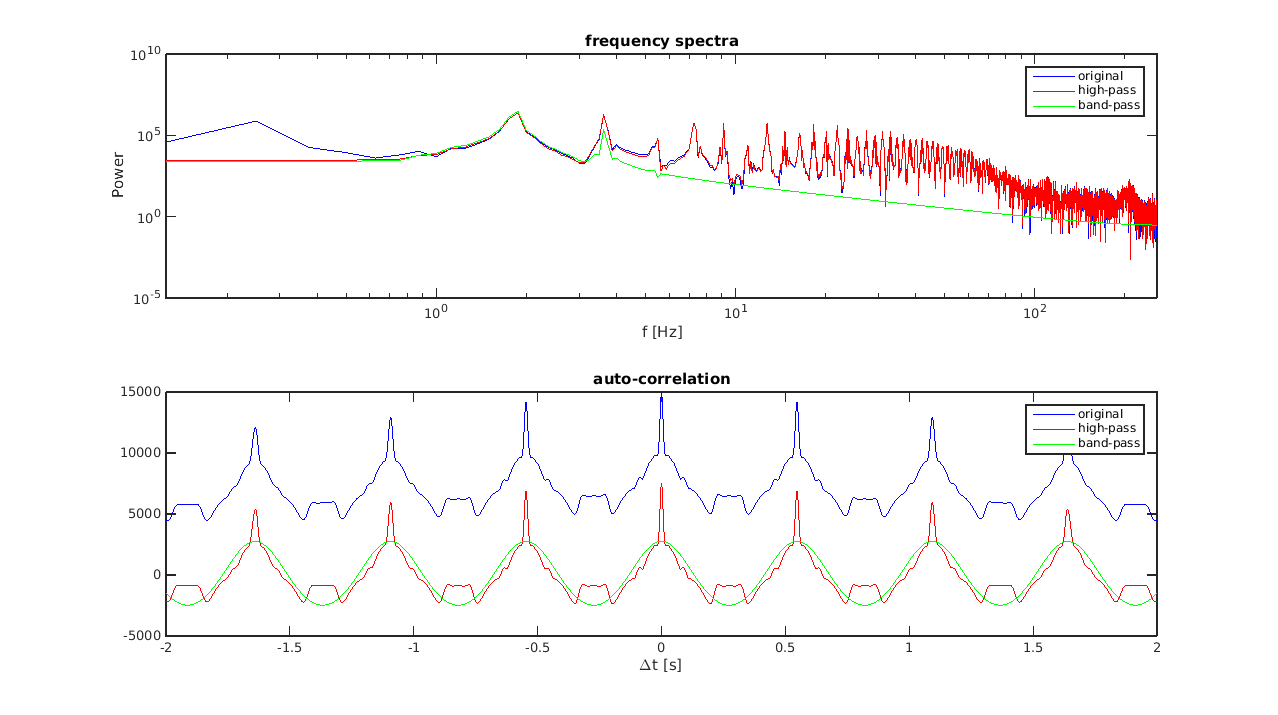
\includegraphics[scale=0.25]{p2fig1.png}
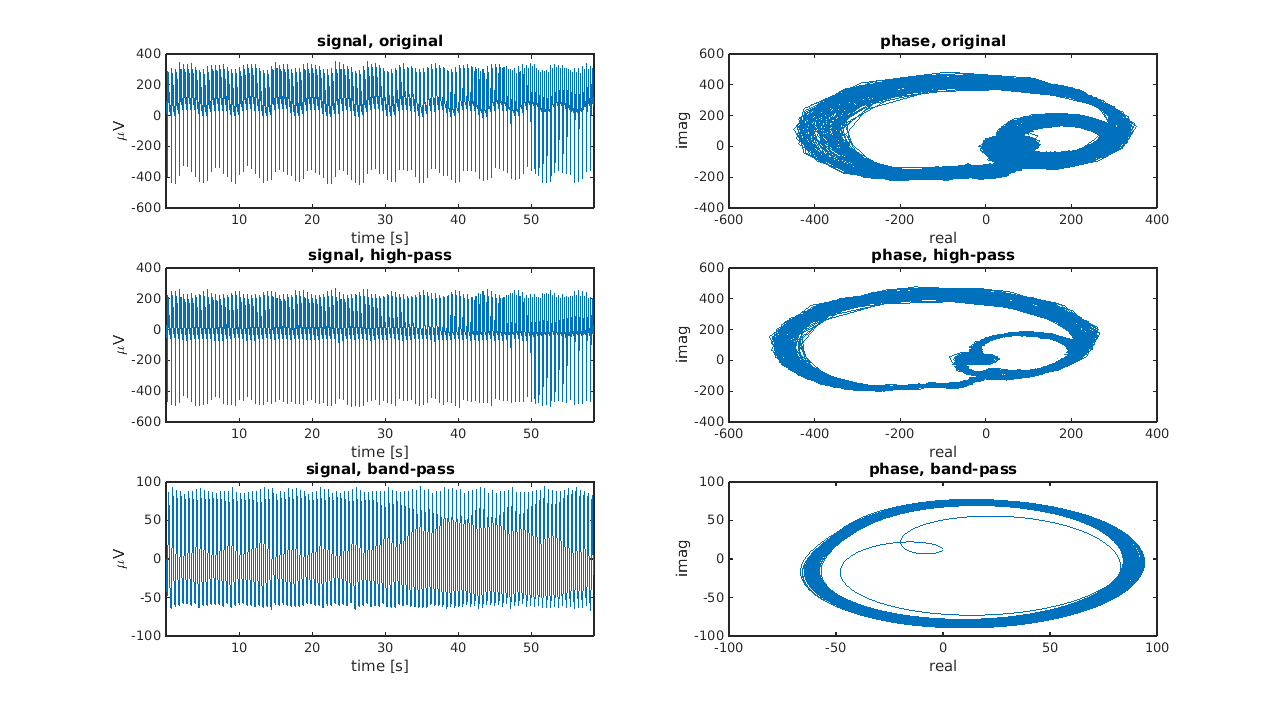
\includegraphics[scale=0.25]{p2fig2.png}

\hspace{-1cm} 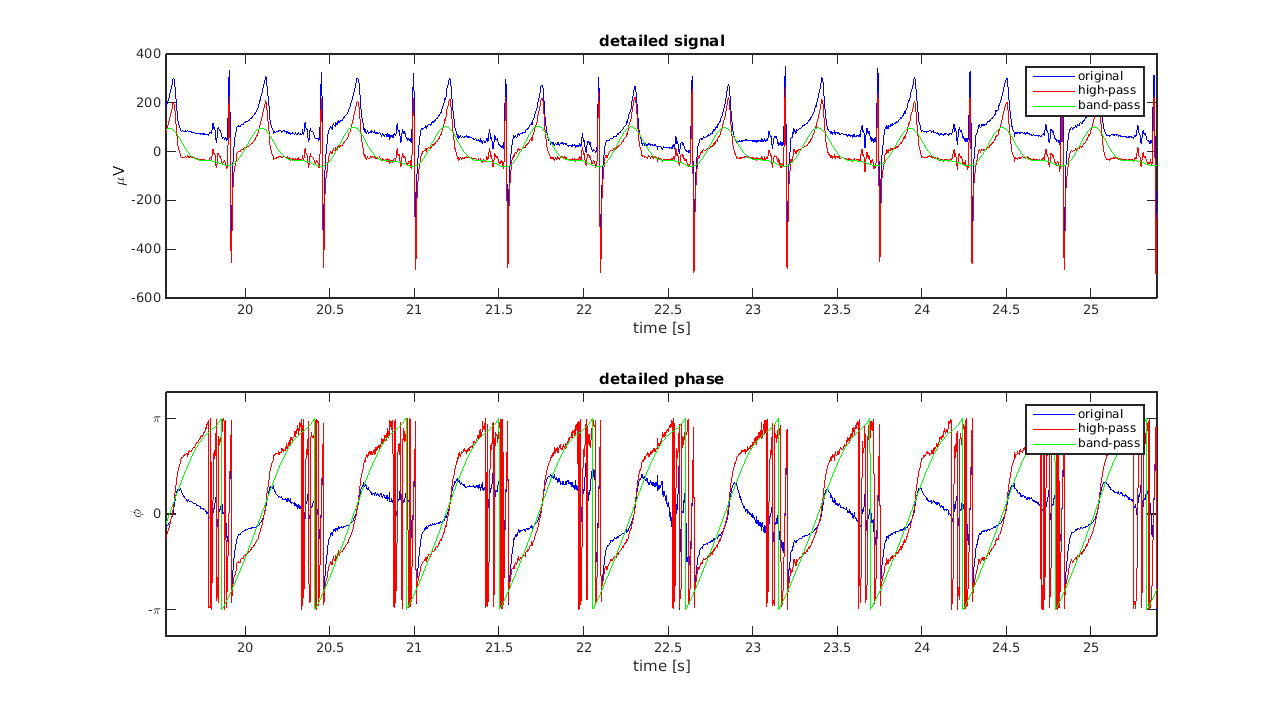
\includegraphics[scale=0.25]{p2fig3.png}
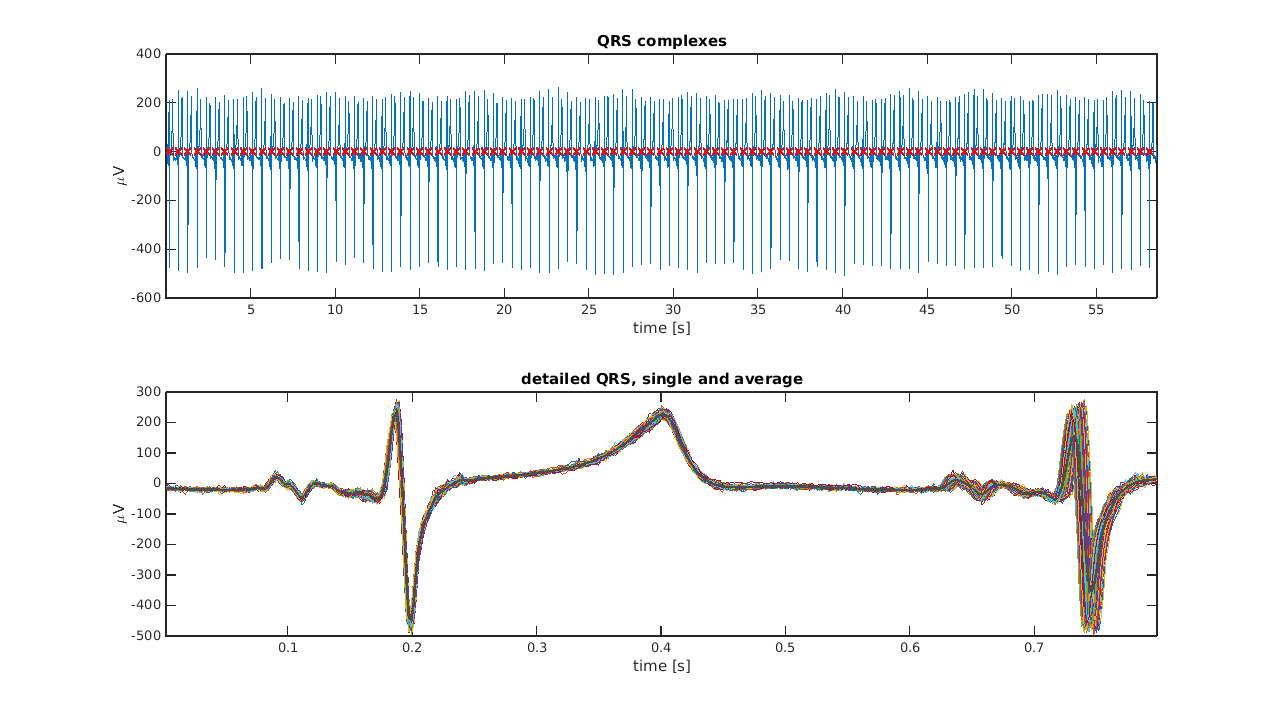
\includegraphics[scale=0.25]{p2fig4.png}

\hspace{-1cm} 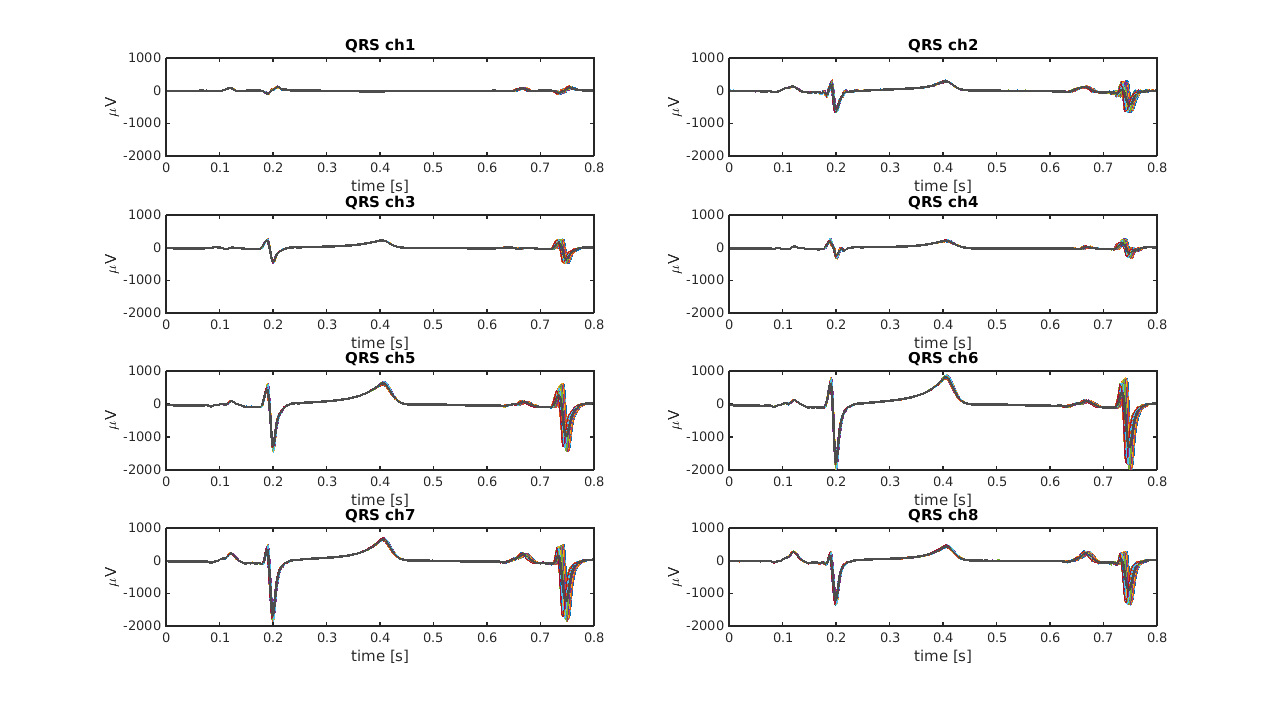
\includegraphics[scale=0.25]{p2fig5.png}
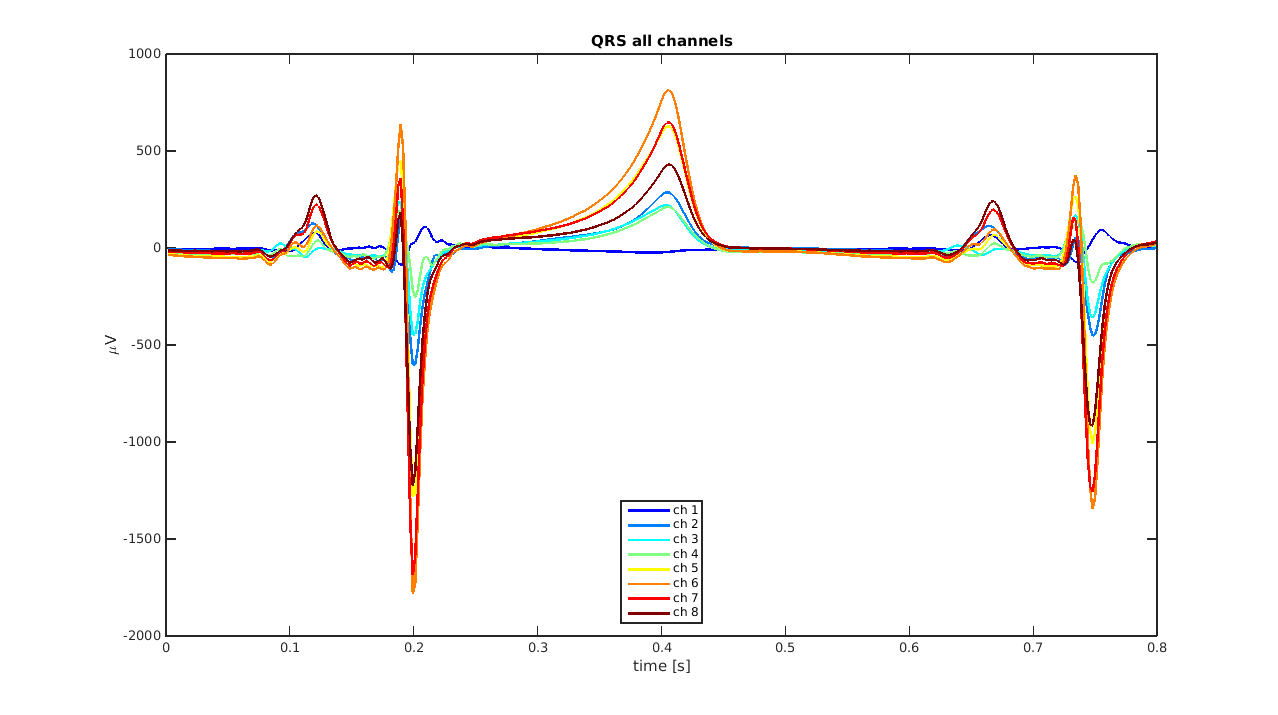
\includegraphics[scale=0.25]{p2fig6.png}


\section*{Part 2}
\texttt{runECG2.m} builds on top of the previous script. We will now look at actual experimental data over 8 blocks of approx. 10 minutes each, recorded at increasing levels of blood dilution. We will only process channel 3 of the data. We specify the sample frequency, load the same filters as before, create some figures, and set the pack size for later computing phase locking values. Then we start iterating over blocks and process each channel 3 signal analogous to the example signal before.

First, we load the signal, filter it, extract QRS peaks, and compute phases. Write the missing code for filtering and computing phases as before. We're only interested in the filtered signals, here.

Next, we epoch the high-pass filtered data. In addition to the signal, you also have to epoch its phase. Use the \texttt{unwrap} function to fold the sawtooth-shaped phase out of the interval $[-\pi, \pi]$, and shift each phase epoch up/down so it crosses zero at the QRS peak position. This way, we make phase progression comparable among sweeps. \texttt{waves} and \texttt{phases} will be of the same size, containing one epoch per column.

Based on the phase, we can now compute the phase locking value (PLV) along the epoch, over consecutive sweeps. In mathematical terms, we will compute the mean phase coherence over all epochs $k$ in pack $P$
\begin{equation*}
PLV_P(t) = \lvert \frac{1}{N}\sum_{k\in P}e^{i\phi_k(t)} \rvert
\end{equation*}
which is obtained for each time $t$ by averaging the normalized complex phase over epochs and then taking the absolute value, which gives the magnitude of phase angle similarity within pack $P$. Try to implement this equation directly in MATLAB. You can process each phase vector $\phi_k$ as a whole, without explicitely iterating over $t$.

That's it. There is nothing to edit in the plotting part. Your code should produce the 4 figures below.

\vspace{1cm}
\hspace{-1cm} 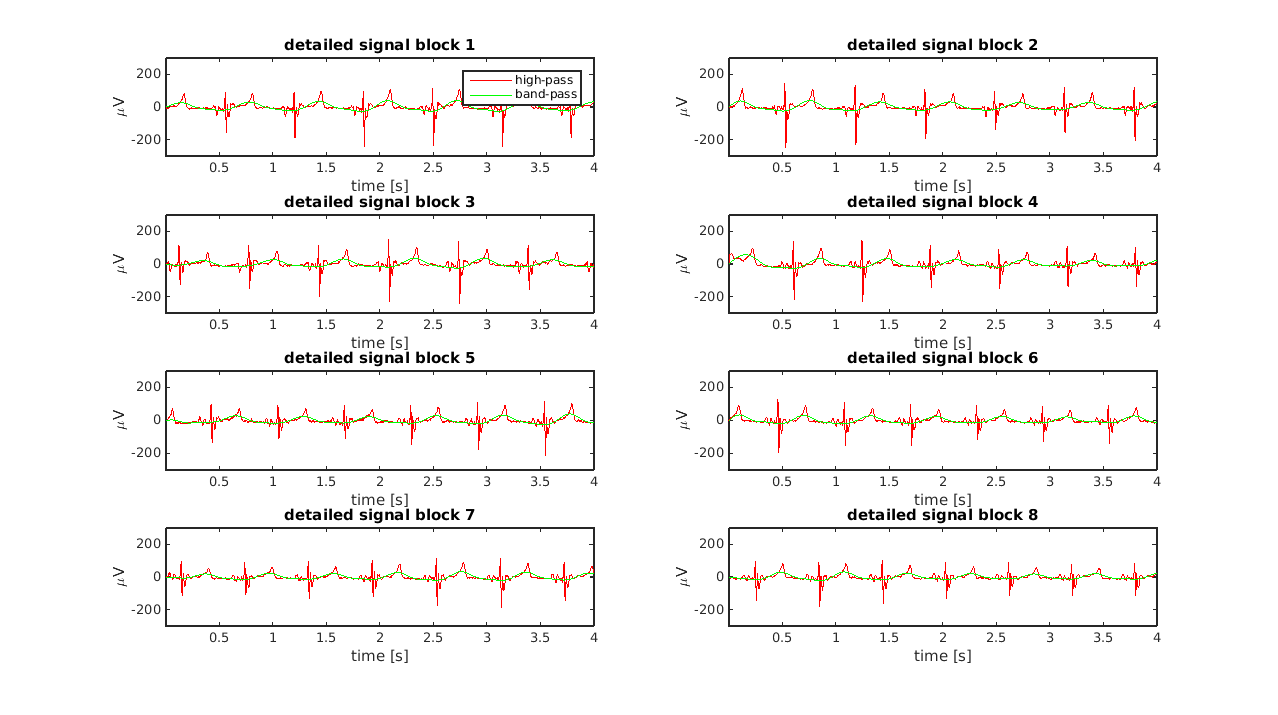
\includegraphics[scale=0.25]{p2fig7.png}
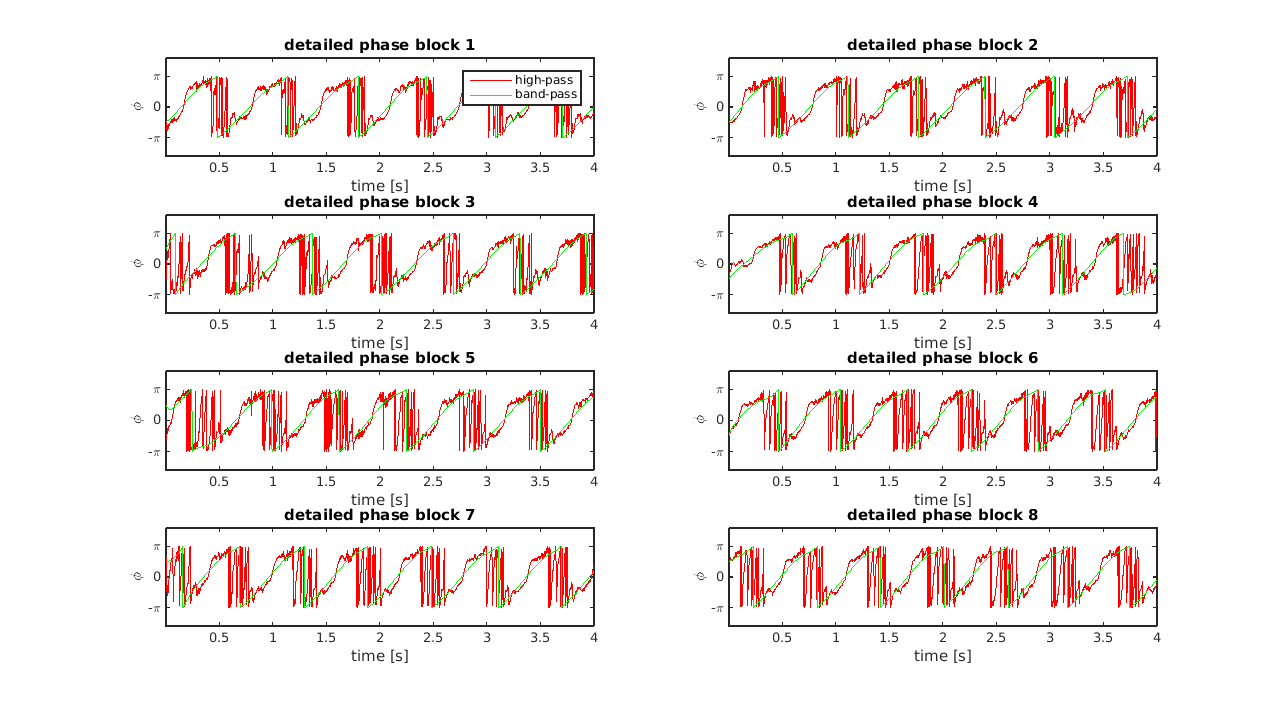
\includegraphics[scale=0.25]{p2fig8.png}

\hspace{-1cm} 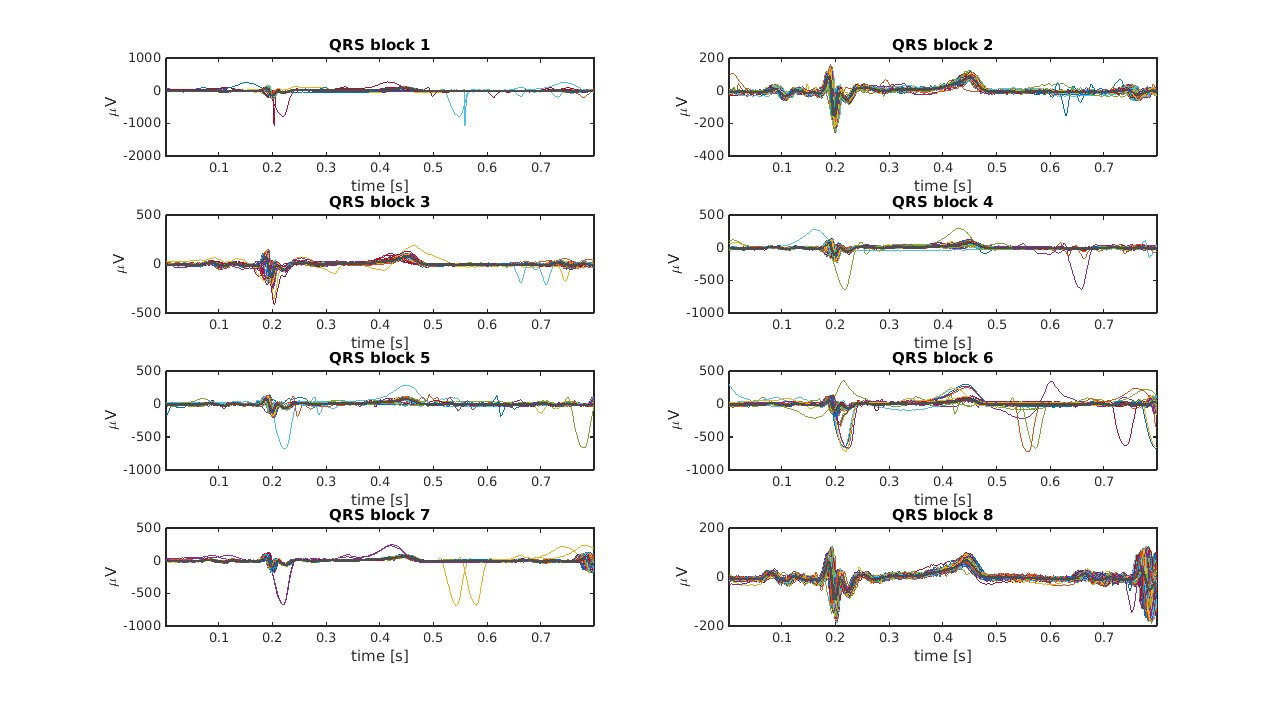
\includegraphics[scale=0.25]{p2fig9.png}
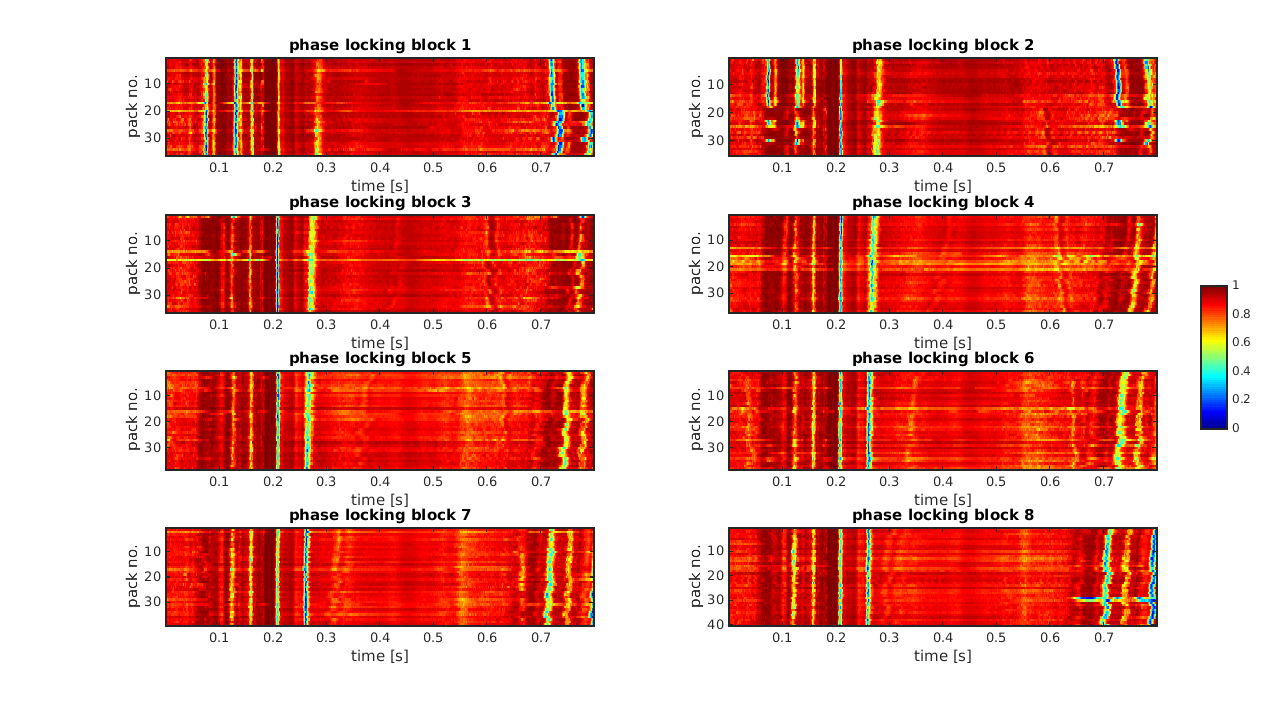
\includegraphics[scale=0.25]{p2fig10.png}
\vspace{5mm}

Compare the signal, phase, and PLV between the 8 levels of blood dilution. Try to identify differences and commonalities between blocks along the epoch. You should leave these figures open when working on the final script.


\section*{Part 3}
In the last part, we want to process 2 out of the 8 blocks and train a classifier on the data. \texttt{runECG3.m} starts as before, in addition specifying the 2 blocks of choice and initializing a variable to store the features (apparently, we're going to compute phases for the high-pass and band-pass filtered signal and phase locking for the high-pass filtered signal).

Fill the gaps in the analysis section of the code. This is almost identical to the previous script. In the end, we have a variable \texttt{Features} containing the 3 feature matrices for each of the two blocks.

Now we want to train and validate a model on these features. The first thing you should do is cut down the number of epochs to a multiple of \texttt{packSize}, because we only have PLVs for the first \texttt{nPacks}*\texttt{packSize} epochs and we don't want to use the remaining, incomplete data. Make sure you consider the minimum \texttt{nPacks} of the two blocks of features as a lower bound. \texttt{useEpochs} should contain the respective indices.

Next, from your previous analyses and Scheller et al. (2011), derive two time points that correspond roughly to the QRS peak and the T wave of the typical epoch. We will use the feature values at these two points for classification. Note that we have set all phases to zero exactly at the QRS peak, so \texttt{t1} has to be a point shortly before or after the actual peak.

We can now construct the feature matrix by iterating over the two blocks and putting the 6 feature values for each epoch in the corresponding row of \texttt{X}. The difficult part here is to correctly elongate the PLV matrix, such that each epoch is assigned the PLV of the pack that it belonged to in the above calculation. Use functions \texttt{reshape} and \texttt{repmat} to produce the elongated matrix, or try iterating explicitely over epochs to make the problem less complex.

Finally, in order to train different models on the data, we have to extend our function \texttt{modelFitVal.m} such that it takes an additional input string to specify the model to use (\texttt{'logreg'}, \texttt{'linsvm'}, or \texttt{'rbfsvm'}) and implements the different training and validation procedures accordingly. Fill the missing parts in \texttt{modelFitVal2.m} to implement the 3 different cases. Find the appropriate functions to train SVMs in the MATLAB documentation.

Your main script \texttt{runECG3.m} should now print the cross-validated performance of each model, which should ideally be above 90 \%. If not, try to improve performance by varying \texttt{t1} and \texttt{t2}, or check your signal processing steps. If all 3 models perform at or below 50 \%, something is seriously wrong (the same goes for exactly 100 \%). Otherwise, you basically solved the problem.

\end{document}
